% !TeX spellcheck = pl_PL
\chapter{Projekt instrumentu muzycznego}
W ramach realizacji projektu konieczne jest zaimplementowanie wielu różnych etapów przetwarzania i sterowania procesem generowania dźwięku: akwizycja sygnałów z klawiatury muzycznej, generowanie dźwięku z procesora DSP oraz komunikacja z interfejsem użytkownika. W niniejszym rozdziale przedstawiono sposób realizacji wymienionych zadań. Omówiono również warstwę sprzętową projektu, odgrywającą podstawową rolę w realizacji syntezatora. Implementacja poszczególnych algorytmów syntezy dźwięku przedstawiona zostanie w kolejnych rozdziałach im dedykowanych.

Kod programu na procesor DSP napisany został w języku C. Program uruchamiano w środowisku Code Composer Studio v6, które jest dedykowane dla procesorów firmy Texas Instruments. Wgrywanie kodu na płytę ewaluacyjną PADK odbywało się poprzez użycie debuggera XDS510 firmy Spectrum Digital.

% zdjęcie PADK z debuggerem

\section{Warstwa sprzętowa instrumentu}
% Zdjęcie i opis co z czym łączymy
Głównymi elementami sprzętu potrzebnymi do realizacji kompletnego instrumentu klawiszowego i jednoczesnego spełnienia założeń projektowych są:
\begin{itemize}
	\item klawiatura MIDI - wysyłanie sygnałów MIDI,
	\item komputer PC - interfejs użytkownika,
	\item płyta uruchomieniowa z procesorem DSP - realizacja podstawowych funkcji instrumentu,
	\item programator DSP,
	\item zestaw nagłośnieniowy.
\end{itemize}

Niniejszy podrozdział poświęcono omówieniu architektury zaprojektowanego instrumentu muzycznego, w którym główną rolę pełni płyta uruchomieniowa procesora DSP.

\subsection{Płyta PADK}
%Dokumentacja plyty PADK: file:///D:/Data/Studia/Magisterka/Z_pendrive/Szefler/Szefler/PADK_LYRTECH/PADK%20-%20Technical%20reference%20guide.pdf
Płyta Professional Audio Development Kit (PADK), która użyta została w niniejszym projekcie, posiada wiele zintegrowanych układów. Dedykowana jest przede wszystkim do testowania aplikacji skupiających się na przetwarzaniu sygnałów dźwiękowych. Głównym jej elementem jest procesor DSP, który łączy ze sobą wszystkie pozostałe podzespoły takie jak: komunikacyjne układy peryferyjne, przetworniki ADC i DAC, układy FPGA oraz interfejs JTAG \cite{dokumentacja_PADK}. Dodatkowo płyta posiada 8MB pamięci flash, 128MB pamięci SDRAM oraz pamięć EEPROM.

\begin{figure}[H]
	\centering
	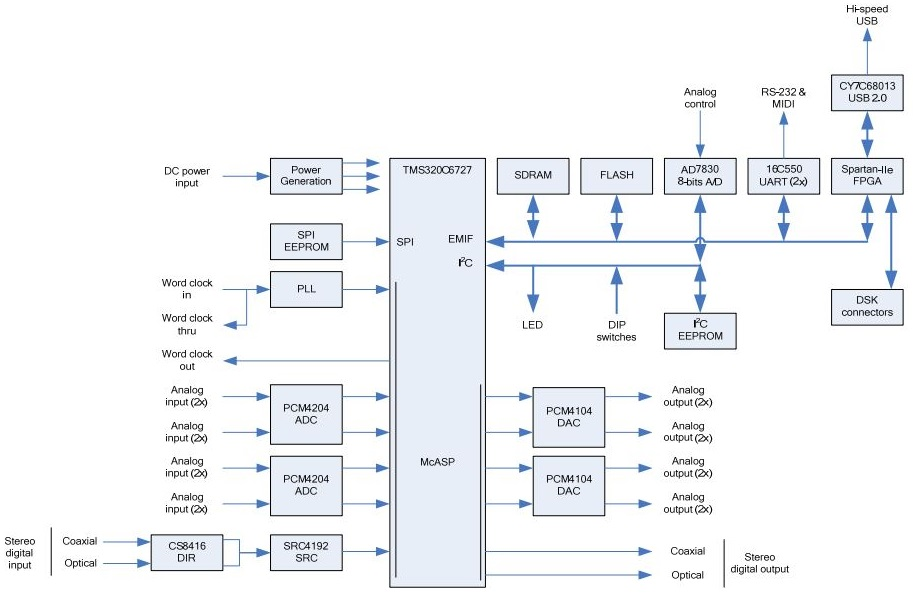
\includegraphics[width=16cm]{./grafiki/real_PADK_block}
	\captionsetup{justification=centering}
	\caption{Schemat blokowy płyty PADK.}
	\label{rys:real_padk}
\end{figure}

Na rysunku \ref{rys:real_padk} przedstawiającym schemat blokowy płyty PADK można zaobserwować uzależnienie układów peryferyjnych od procesora DSP, będącego głównym elementem systemu.

\subsection{TMS320C6727}
%https://www.ti.com/lit/ds/symlink/tms320c6727.pdf?ts=1595978326019&ref_url=https%253A%252F%252Fwww.google.com%252F 
%--> glowne feature'y
%--> strona 13 wypisane w myslnikach np busy
Układ TMS320C6727 firmy Texas instrument jest zmiennoprzecinkowym procesorem sygnałowym 32-/64-bitowym umieszczonym na płycie PADK. Jednostka centralna C6727 posiada możliwość taktowania zegara z szybkością 300MHz oraz 350MHz. Gdy ustawiona jest częstotliwość 300MHz, procesor posiada maksymalną wydajność sięgającą 180 milionów operacji zmiennoprzecinkowych na sekundę \cite{dokumentacja_ti6727}.

Układ TMS320C6727 jest również bardzo wydajny pod względem systemu pamięci. Posiada on 256KB pamięci RAM oraz 384KB pamięci ROM. Kontroler pamięci obsługuje jednocyklowe dostępy z procesora do pamięci  RAM lub ROM. W jednym momencie dozwolone są trzy równoległe odczyty pamięci z różnych źródeł takich jak: CPU, pamięć programu cache oraz jedno z urządzeń peryferyjnych. Układ TMS320C6727 posiada również 32KB pamięci cache programu.

Poza wysoką szybkością taktowania procesora, układ zawiera dodatkowe mechanizmy akceleracji przepływu danych i sygnałów. Umożliwiają one jeszcze szybszy transfer danych między układami peryferialnymi bez zabierania czasu pracy procesora. Narzędzia, z których szczególnie korzystano w naszym projekcie przedstawiono poniżej.

\subsubsection{McASP}
%https://www.ti.com/lit/an/sprack0/sprack0.pdf?ts=1595842361762&ref_url=https%253A%252F%252Fwww.google.com%252F
McASP to akronim od Multichannel Audio Serial Port. Jest to komunikacyjne urządzenie peryferyjne dedykowane do przetwarzania danych audio lub wideo. Zostało zaprojektowane dla wielokanałowego przetwarzania dźwięku. Jedną z najbardziej przydatnych właściwości narzędzia McASP jest możliwość niezależnego taktowania urządzeń podłączonych jednocześnie do magistrali. McASP pozwala na zachowanie niezależności pomiędzy portami odbierającymi i nadającymi. Komunikacja, którą zarządza omawiany protokół może odbywać się poprzez interfejs I2S (ang. Inter-IC Sound), I2C (ang. Inter-Integrated Circuit) lub SPI (ang. Serial Peripheral Interface) \cite{dokumentacja_mcasp}.

Kiedy dane przepływają przez McASP, mogą zostać dostosowane tak, aby reprezentacja stałoprzecinkowa używana przez kod aplikacji była niezależna od reprezentacji używanej przez urządzenia zewnętrzne, bez wymagania dodatkowej konwersji przez procesor.
W niniejszej pracy narzędzie McASP stosowane jest do przepływu danych między DAC a procesorem. 

\subsubsection{dMAX} \label{par:dMax}
%https://www.ti.com/lit/ug/spru795d/spru795d.pdf?ts=1595843361787&ref_url=https%253A%252F%252Fwww.google.com%252F, strona 14, Overview
Kontroler dMAX (Dual Data Movement Accelerator) obsługuje transfery zaprogramowane przez użytkownika pomiędzy kontrolerem pamięci wewnętrznej a urządzeniami peryferialnymi na procesorach DSP firmy Texas Instruments. Mechanizm ten jest dedykowany szczególnie dla procesorów z serii C672x.

Zasada działania dMAX opiera się na sygnałach zdarzeń (ang. event signals). Zdarzenie zdefiniowane jest jako zmiana wartości logicznej odpowiadającego sygnału zdarzeń w rejestrze flag zdarzeń. Zdarzenie może być używane jako: wzbudzenie rozpoczęcia transferu danych lub spowodowane wystąpieniem przerwania dla CPU. Wszystkie zdarzenia posortowane są w dwie grupy: niskiego oraz wysokiego priorytetu. Mechanizm dMAX może równolegle przetwarzać dwa żądania zdarzeń z każdej z grupy \cite{dokumentacja_dmax}.

Częścią mechanizmu dMAX jest również bufor cyrkulacyjny FIFO. Pozwala on na równoczesny, asynchroniczny odczyt i zapis danych do jednego bufora dwustronnego. Narzędzie dMAX wykrywa kiedy dane zostają zapisane do bufora i natychmiastowo wywołuje odwrócenie go. Po odwróceniu, zapisane chwilę wcześniej dane mogą zostać odczytane z drugiej strony bufora, natomiast równocześnie, kolejne dane są zapisywane po pierwszej stronie.

\subsection{Peryferia komunikacyjne}
Płyta PADK ma możliwość komunikowania się z innymi urządzeniami przez trzy różne interfejsy:
\begin{itemize}
	\item UART,
	\item MIDI,
	\item USB.
\end{itemize}
Za komunikację przez interfejs MIDI oraz UART odpowiadają dwa układy TL16C550. Pozwalają one na alternatywny tryb kolejki danych FIFO, który odciąża procesor DSP. Interfejs USB obsługiwany jest na płycie poprzez mikrokontroler CY7C68013.

\subsection{Przetworniki DAC}
Na płycie PADK znajdują się dwa, czterokanałowe, 24-bitowe układy PCM4204, które posiadają możliwość próbkowania sygnału z częstotliwością do 192kHz. Umożliwiają one odczyt z płyty uruchomieniowej analogowegych sygnałów dźwiękowych za pomocą gniazd żeńskich typu CINCH.

\subsection{Pełen schemat układu instrumentu klawiszowego}
\begin{figure}[H]
	\centering
	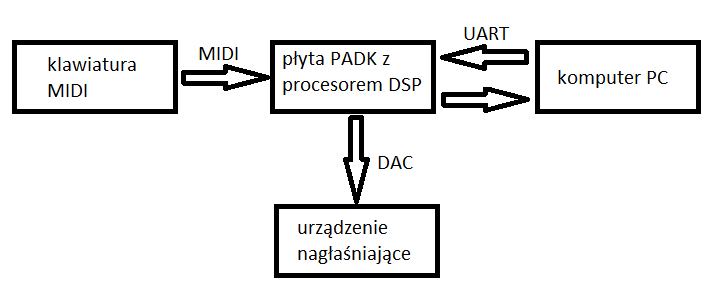
\includegraphics[width=12cm]{./grafiki/real_pelen_uklad}
	\captionsetup{justification=centering}
	\caption{Schemat pełnego układu realizowanego w projekcie.}
	\label{rys:real_uklad}
\end{figure}
Strzałki na rysunku \ref{rys:real_uklad} przedstawiają kierunek przepływu danych między głównymi elementami projektowanego układu. Klawiatura MIDI komunikuje się z płytą PADK za pomocą protokołu MIDI. Komputer osobisty z interfejsem użytkownika służy do dwukierunkowej komunikacji z płytą uruchomieniową z wykorzystaniem interfejsu UART. Ostatecznie płyta PADK przesyła próbki dźwięków do przetwornika DAC, którego wyjście analogowe jest połączone z zestawem nagłośnieniowym. Zestaw pozwala odsłuchiwać zsyntezowane brzmienia.

\section{Komunikacja z płytą PADK}
Do oprogramowania płyty PADK dołączone zostały dodatkowe biblioteki firmy Lyrtech, które ułatwiają obsługę jej komunikacji z urządzeniami zewnętrznymi. Przykładem interfejsów, dla których zostały utworzone nadmienione biblioteki, są UART oraz MIDI.

Inicjalizacja przerwań i transferu danych obu interfejsów wygląda bardzo podobnie. Każdy z nich otrzymał swój identyfikator zdarzenia dMAX oraz identyfikator przerwania. Priorytet przerwań obu interfejsów ustawiono na wysoki. Ostatnim elementem inicjalizacji układów było ustawienie rejestru IER obu interfejsów na wartość umożliwiającą pracę w trybie przerwań.

\subsection{Komunikacja z klawiaturą muzyczną  (MIDI)}
% Datasheet "Professional Audio Development Kit Technical Reference Guide 1.4", September 2007
Klasyczny interfejs klawiatury MIDI jest wyposażony w pięciopinowe gniazdo DIN. Na płycie PADK zastosowano jednak dziewięciopinowe gniazdo typu D-sub. Z tego powodu, aby połączyć klawiaturę muzyczną z płytą PADK, należało zbudować kabel z odpowiednimi wtykami.

Do obsługi interfejsu MIDI wykorzystana została biblioteka PADK\_MIDI.c, która zawiera takie funkcje jak:
\begin{itemize}
	\item MIDI\_Init - inicjalizacja interfejsu MIDI,
	\item MIDI\_EnableLed1, MIDI\_EnableLed2 - sterowanie diodami LED interfejsu MIDI,
	\item MIDI\_Read - odczyt przychodzących bajtów. 
\end{itemize}
W celu jak najmniejszego zużycia czasu procesora, obsługa interfejsu MIDI została sprowadzona jedynie do odczytywania przychodzących bajtów poprzez przerwania sprzętowe.
Jako że ramki MIDI składają się z trzech bajtów, odczytywać oraz interpretować należy kolejne 3 przychodzące bajty.
Można to osiągnąć poprzez umieszczenie funkcji MIDI\_Read z parametrem 3 - przerwanie sprzętowe co każde odczytane 3 bajty. Sytuację nieco komplikuje zegar MIDI pojawiający się "losowo", który powoduje, że DSP odczytuje regularnie bajt o wartości 0xF8 zakłócających odczytanie użytecznych danych MIDI. Powoduje to, że w odczytanej sekwencji 3 bajtów pojawiała się niepożądana wartość 0xF8.
\begin{figure}[H]
	\centering
	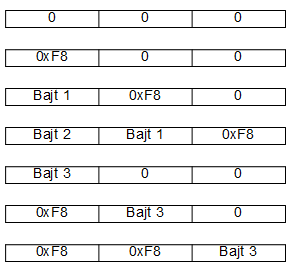
\includegraphics[width=8cm]{./grafiki/real_nofifo}
	\captionsetup{justification=centering}
	\caption{Odczytywane ramki MIDI przy braku odpowiedniej procedury odczytu.}
	\label{rys:real_nofifo}
\end{figure} 
Problem ten został zobrazowany na rysunku \ref{rys:real_nofifo}. Przedstawia on zawartość bufora wejściowego w czasie biegnącym od góry do dołu rysunku. W pokazanej sytuacji pomiędzy wywołaniem funkcji MIDI\_Read z parametrem 3, a nadejściem 3-bajtowej ramki danych, został odczytany bajt zegarowy. Ostatecznie odczytana zostanie ramka czwarta oraz siódma od góry.  Oznacza to, że bajty, które miały zostać odczytane jako jedna ramka, mogą być dowolnie rozbite pomiędzy dwa wywołania ISR. 
Aby rozwiązać ten problem, ISR wywołuje funkcję MIDI\_Read z parametrem 1. W rezultacie każdy przychodzący bajt wywołuje przerwanie. W jego obsłudze sprawdzana jest wartość bajta, jesli jest ona różna od 0xF8 (zegar MIDI), to zostaje ona dodana do trzyelementowej kolejki FIFO. W momencie gdy kolejka FIFO się zapełnia, ramka jest identyfikowana i interpretowana, a kolejka czyszczona. Działanie takiej kolejki zobrazowane jest na rysunku \ref{rys:real_fifo}.
\begin{figure}[H]
	\centering
	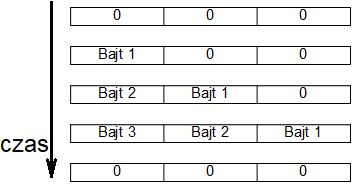
\includegraphics[width=8cm]{./grafiki/real_fifo}
	\captionsetup{justification=centering}
	\caption{Odczytywane ramki MIDI przy wykorzystaniu kolejki FIFO odrzucającej bajty zegarowe.}
	\label{rys:real_fifo}
\end{figure} 
Dzięki sprawdzaniu każdego przychodzącego bajta w obsłudze przerwania, do kolejki FIFO dostają się tylko istotne bajty. Dyskryminowanie wartości 0xF8 nie powinno mieć skutków ubocznych, gdyż wartość ta nie pojawia się w żadnym z bajtów ramki MIDI, poza bajtem statusu komunikatu zegarowego.

\subsection{Komunikacja z interfejsem użytkownika (UART)}
Do komunikacji płyty PADK z panelem sterującym użytkownika działajacym na komputerze klasy PC wykorzystany został interfejs RS-232. Aby umożliwić komunikację komputera nie posiadającego wyżej wymienionego interfejsu wykorzystano układ konwertujący RS-232 na USB.

Do obsługi protokołu szeregowego została wykorzystana biblioteka PADK\_UART.c, która zawiera takie funkcje jak:
\begin{itemize}
	\item UART\_Init - inicjalizacja interfejsu UART,
	\item UART\_EnableLed1, UART\_EnableLed2 - sterowanie diodami LED interfejsu UART,
	\item UART\_Read - odczyt przychodzących bajtów,
	\item UART\_Write - nadanie bajtów.
\end{itemize}
Aby zapewnić wygodny w użyciu oraz odporny na błędy przepływ informacji, utworzono własny protokół.
\begin{figure}[H]
	\centering
	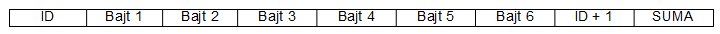
\includegraphics[width=16cm]{./grafiki/real_uartframe}
	\captionsetup{justification=centering}
	\caption{Struktura ramki protokołu.}
	\label{rys:real_uartframe}
\end{figure}
Na rysunku \ref{rys:real_uartframe} pokazana została struktura 9-bajtowej ramki danych, która jest przesyłana pomiędzy DSP a komputerem. Składa się ona z dwóch bajtów identyfikujących, sześciu bajtow danych oraz jednego bajta sumy kontrolnej. Podobnie jak w przypadku MIDI, do identyfikacji i interpretacji przychodzących ramek, wykorzystywana jest kolejka FIFO. Tym razem ma ona rozmiar 9 bajtów. Bajty przychodzące są odczytywane pojedynczo przy wykorzystaniu przerwania sprzętowego i wpisywane do kolejki FIFO. W momencie gdy na pierwszym miejscu w kolejce znajdzie się odpowiedni bajt identyfikujący ramkę, a na miejscu ósmym znajdzie się jego wartość powiększona o jeden, można zakładać, że odebrana została "jakaś" ramka danych. W celu potwierdzenia jej poprawności, obliczana jest suma kontrolna z bajtów danych. Gdy ramka przejdzie taką weryfikację, zostaje odczytana informacja, którą niesie. Opisany mechanizm działa zarówno na procesorze DSP, jak i na komputerze PC.
Takie dziewięciobajtowe ramki pozwalają na przesyłanie na przykład całych zmiennych 4-bajtowych lub jednocześnie trzech liczb 2-bajtowych. 



\section{Generowanie sygnału analogowego (DAC)}

\subsection{Inicjalizacja programowa modułu DAC}
Odpowiednie zainicjowanie pracy przetwornika cyfrowo analogowego było najbardziej skomplikowanym elementem etapu uruchomienia całego projektu. Polegało ono na:
\begin{itemize}
\item ustawieniu identyfikatora zdarzeń dMAX, 
\item zdefiniowaniu przerwania dedykowanego dla DAC, 
\item ustawieniu bitów rejestrów modułu McASP
\item przydzieleniu odpowiedniego obszaru pamięci,
\item dobraniu parametrów dla przetwornika DAC.
\end{itemize}
%pamiętać o: odniesienie do dMAX z buforem cyrkulacyjnym
%pamięć dla bufora
%źródła zegarów
%parametry

Program dotyczący modułu DAC wykorzystuje bufor cyrkulacyjny, którego działanie omówiono w \ref{par:dMax}. Pierwszym elementem inicjalizacji było ustawienie odpowiedniego obszaru pamięci dla zmiennej z buforem cyrkulacyjnym dmaxDacBuffer[PING/PONG][FRAME][L/R][.]. Następnie w programie ustawiono źródła zegarów taktujących przetwornik DAC. Kolejnym krokiem była inicjalizacja parametrów dla przetwornika. Tryb szybkości próbkowania ustawiony został na najwolniejszy, obejmujący szybkości 32kHz, 44,1kHz oraz 48kHz. Ustawiono rejestr odblokowujący generowanie sygnału z przetwornika oraz format danych na 24 bitowy wyjustowany do lewej (ang. left-justified). 
% Wytlumaczyc to left-justified - ze w liczbie 32 bitowej traci sie 8 bitów
Priorytet przerwania został ustawiony na wysoki. Wszystkie wartości zostały przekazane za pomocą funkcji z bibliotek firmy Lyrtech o nazwie DAC\_Init().


% DMAX for data transfer on MCASP0TX DMA REQ - 3D Transfer
% DMAX Parameter initialization structure
% DMAX Event initialization structure
Kolejnym etapem była inicjalizacja parametrów dotyczących połączenia przetwornika cyfrowo-analogowego z modułem McASP oraz ustawienia struktury zdarzenia dMAX powiązanego z przetwornikiem DAC. 

Ostatnią częścią inicjalizacji było ustawienie częstotliwości próbkowania na wartość 48kHz i wyłączenie przekaźnika blokującego przepływ sygnału analogowego z przetwornika do gniazda CINCH.

\subsection{Komunikacja między procesorem a przetwornikiem DAC}
Obsługa danych zawierających zsyntezowane dźwięki oraz ich przesłanie na moduł DAC odbywa się za pomocą przerwania dmax\_isr(). Za każdym razem, gdy wywoływane jest przerwanie z wykorzystaniem zdarzenia dMAX, sprawdzany jest warunek, czy poprzedni transfer danych na przetwornik DAC został ukończony. Jeżeli warunek jest spełniony, pozostały kod funkcji obsługi przerwania zostaje wykonany.

Obsługa danych tej funkcji opiera się na zainicjalizowanym wcześniej buforze cyrkulacyjnym dmaxDacBuffer[PING/PONG][FRAME][L/R][.]. Programowo bufor jest czterowymiarową tablicą, gdzie pierwszy wymiar dokonuje synchronizacji odczytu i zapisu typu ping-pong. Następnie wykonywany jest mechanizm zakładkowania dwóch tablic przechowujących próbki zsyntezowanego dźwięku. Dane po zakładkowaniu przekazywane są do modułu DAC przez tablicę dmaxDacBuffer[PING/PONG][FRAME][L/R][.].

\section{Klawiatura polifoniczna}\label{section:real_polifonia}
Jednym z wymagań projektowych jest implementacja polifonii. Generowanie więcej niż jednego tonu jednocześnie zostało osiągnięte poprzez asynchroniczne odczytywanie wciśnięć i zwalniania klawiszy instrumentu oraz przechowywanie informacji o klawiszach wciśniętych w danej chwili. Rozwiązano to poprzez utworzenie tablicy freqs[.] o 12 elementach typu float (zakłada się obsługę nie więcej niż 12 klawiszy jednocześnie). Odebranie ramki MIDI z informacją o wciśnięciu klawisza instrumentu, powoduje wpisanie odczytanej wartości częstotliwości do niezajętej komórki tablicy. Gdy dźwięk związany z danym klawiszem kończy wybrzmiewanie, odpowiedni element tablicy jest zerowany. W każdej z metod syntezy odczytywane są częstotliwości z tej tablicy i generowane odpowiednie dźwięki. Rozwiązania polifonii różnią się pomiedzy metodami syntezy, z tego powodu zostaną one indywidualnie opisane w odpowiednich rozdziałach.
% opisać ogólnie, i powiedziec, ze dla kazdej metody to bedzie wyglądało trochę inaczej



\section{Wykorzystanie algorytmu FFT}
%http://www.secs.oakland.edu/~ganesan/old/courses/CSE671SU08/CSE%20671%20Lab%204%20ANC%20Code/Lee's%20adaptive%20wiener%20filter/DSPF_sp_cfftr2_dit.h

%https://processors.wiki.ti.com/index.php/C674x_DSPLIB <--- funkcje dsp_lib

W pamięci ROM procesorów z serii TMS320C672x zostały umieszczone specjalnie zoptymalizowane biblioteki, dedykowane do szybkiego przetwarzania sygnałów cyfrowych. Skompilowane biblioteki zostały napisane w asemblerze w celu większej efektywności obliczeniowej. 

%https://www.ti.com/lit/an/spraas8/spraas8.pdf?ts=1596035199216&ref_url=https%253A%252F%252Fwww.google.com%252F
W autorskim projekcie została użyta biblioteka \emph{DSP Library} z procesora TMS320C6727, która posiada efektywne obliczeniowo funkcje takie jak: transformacja FFT, odwracanie macierzy lub operacje na wektorach. W celu wykorzystania jej w programie dla DSP, należało zmodyfikować komende pliku linkera, dodając bibliotekę o nazwie \emph{c67xdsplibR.lib}. Dodatkowo zmieniono sekcję pamięci tak, aby linker został odpowiednio poinstruowany, do których obszarów pamięci powinien się odnieść. Do pełnej transformacji FFT użyto trzech funkcji: DSPF\_sp\_cfftr2\_dit(), DSPF\_sp\_icfftr2\_dif() oraz DSPF\_sp\_bitrev\_cplx().

\subsection{Funkcje zawarte w pamięci ROM procesora}
%http://software-dl.ti.com/jacinto7/esd/processor-sdk-rtos-jacinto7/latest/exports/docs/dsplib_c66x_3_4_0_0/docs/doxygen/html/dsplib_html/group___f_f_t.html
Funkcja DSPF\_sp\_cfftr2\_dit() odpowiada za przeprowadzenie algorytmu FFT radix-2 z decymacją w dziedzinie czasu dla liczb zmiennoprzecinkowych. Sygnał na wejściu powinien posiadać N liczb zespolonych ułożonych w tablicy kolejno w pary liczb rzeczywistych i urojonych. Jako drugi argument wejściowy funkcja przyjmuje tablicę współczynników obrotu dla FFT o długości N/2. Współczynniki obrotu utworzone zostają przez zestaw trzech funkcji udostępnionych na stronie producenta procesora. Funkcje zostały skopiowane do autorskiego projektu. %https://www.rose-hulman.edu/class/ee/yoder/ece581/TI%20library/C6700/dsplib/support/fft/tw_r2fft.c <-- twiddle factors
Według dokumentacji opisywana funkcja może również zostać użyta do uzyskania transformaty odwrotnej, poprzez zmianę kolejności współczynników obrotu, a na końcu podzielenie wynikowej transformaty przez N. Jest to działanie odpowiadające wzorowi (\ref{equ:idft_upr}). Wyniki zastosowania funkcji DSPF\_sp\_cfftr2\_dit() jako odwrotnej transformacji okazały się błędne. W celu poprawienia wyników, zastosowano funkcję DSPF\_sp\_icfftr2\_dif(), która dedykowana jest konkretnie do odwrotnej transformacji DFT. Wykonuje ona algorytm FFT radix-2 z decymacją w dziedzinie częstotliwości. Po użyciu tej funkcji, wyniki były poprawne.

%http://software-dl.ti.com/jacinto7/esd/processor-sdk-rtos-jacinto7/latest/exports/docs/dsplib_c66x_3_4_0_0/docs/doxygen/html/dsplib_html/group___d_s_p_f__sp__bitrev__cplx.html
Za zmianę kolejności próbek w tablicy wynikowej otrzymanej z funkcji wykonującej algorytm FFT odpowiada funkcja DSPF\_sp\_bitrev\_cplx(). Zmiana ciągu elementów tablicy realizowana jest przez odczytanie jej indeksów jako liczb w postaci bitowej, a następnie dokonanie lustrzanego odbicia każdego indeksu z osobna (ang. bit-reverse). Jest to niezbędny krok do zrealizowania pełnego algorytmu FFT radix-2.

\subsection{Pełna realizacja algorytmu przekształcenia}
Pełne wykorzystanie algorytmu wymagało odpowiedniego ułożenia omówionych wyżej funkcji. W tym celu utworzono bibliotekę z dodatkowymi funkcjami, które wykonują pełne przekształcenie DFT za pomocą algorytmu FFT. Funkcje dostępne dla użytkownika to fft\_full() oraz ifft\_full(). Pierwsza z nich ustawia funkcję w kolejności:
\begin{enumerate}
	\item bitrev\_full() - generacja współczynników obrotu, przygotowanie próbek dla algorytmu FFT,
	\item DSPF\_sp\_cfftr2\_dit() - wykonanie algorytmu FFT radix-2 z decymacją w dziedzinie czasu,
	\item DSPF\_sp\_bitrev\_cplx() - zmiana kolejności próbek po wykonaniu funkcji FFT,
\end{enumerate}
i pozwala na wykonanie pełnego przekształcenia prostego DFT. Natomiast druga, wykorzystuje funkcje:
\begin{enumerate}
	\item DSPF\_sp\_bitrev\_cplx() - generacja współczynników obrotu, przygotowanie próbek dla algorytmu FFT,
	\item DSPF\_sp\_icfftr2\_dif() - wykonanie algorytmu FFT radix-2 z decymacją w dziedzinie częstotliwości,
\end{enumerate}
do odwrotnego przekształcenia DFT.

% o rozdzielczości
% https://www.bitweenie.com/listings/fft-zero-padding/
\subsection{Rozdzielczość częstotliwości}
Jednym z elementów projektowania układów cyfrowego przetwarzania sygnałów jest odpowiednie dobranie ilości próbek do pojedynczej transformacji DFT. W związku z użyciem algorytmu FFT typu radix-2, liczba próbek musi być potęgą dwójki. Powiązanie autorskiej pracy z dziedziną syntezy dźwięku wymaga również wysokiej dokładności w dziedzinie częstotliwości, aby móc tworzyć tony z dużą dokładnością. Miarą dokładności jest rozdzielczość częstotliwości (ang. frequency resolution), która określana jest wzorem:

\begin{equation} \label{equ:fft_resol}
\Delta R = \frac{f_{s}}{N_{fft}}
\end{equation}
\begin{tabular}{ l l l l}
	gdzie: 	&	$\Delta R$ & - &  rozdzielczość częstotliwości, \\
	&	$f_{s}$ & - &  częstotliwość próbkowania, \\
	&   $N_{fft}$ &  - & liczba punktów transformacji DFT. \\
\end{tabular}

% http://cds.cern.ch/record/720344/files/ab-note-2004-021.pdf
W literaturze można znaleźć informacje, iż widmo częstotliwościowe jest dużo bardziej dokładne przy większej rozdzielczości częstotliwości. Minusem jej zwiększenia jest jednak spowolnienie obliczenia transformaty wynikowej i tym samym negatywny wpływ na czas wykonania programu na procesorze.

%Potwierdzenie ze jak sie zwiekszy rozdzielczosc to jest lepiej https://ieeexplore-1ieee-1org-10000074b15d2.han.bg.pg.edu.pl/document/1604324
Podjęto próby osiągnięcia jak największej rozdzielczości DFT na wykorzystywanym procesorze TMS320C672x. Dokumentacja funkcji realizującej algorytm FFT wskazywała, iż liczba próbek do jednokrotnej transformacji DFT powinna wynosić maksymalnie 2048. Po wprowadzeniu takiej wartości, procesor ulegał zawieszeniu. Obniżenie liczby próbek do 1024 pozwoliło na bezproblemowe działanie procesora. Jednocześnie spowodowało ono dwukrotne obniżenie dokładności. Ze wzoru (\ref{equ:fft_resol}) można wyliczyć, iż rozdzielczość częstotliwości w autorskim projekcie wyniosła 46,875Hz.


\section{ADSR}
Kształtowanie obwiedni generowanych dźwięków związane jest z naciskaniem i zwalnianiem klawiszy syntezatora. Realizacja ADSR'a musi uwzględniać założenie, że klawisze nie muszą być naciskane równocześnie. Fakt ten wyklucza zastosowanie jednego globalnego systemu kształtowania obwiedni. Zastosowanym rozwiązaniem jest kształtowanie obwiedni dla każdego klawisza indywidualnie. Doprowadziło to do powstania dwóch 12 elementowych tablic:
\begin{itemize}
	\item tablica typu float, która przechowuje aktualną wartość obwiedni dla wybrzmiewających dźwięków,
	\item tablica typu int, która przechowuje stan ADSR dla wybrzmiewających dźwięków.
\end{itemize}
Poszczególne stany ADSR zaznaczone zostały na rysunku \ref{rys:real_adsr}.
\begin{figure}[H]
	\centering
	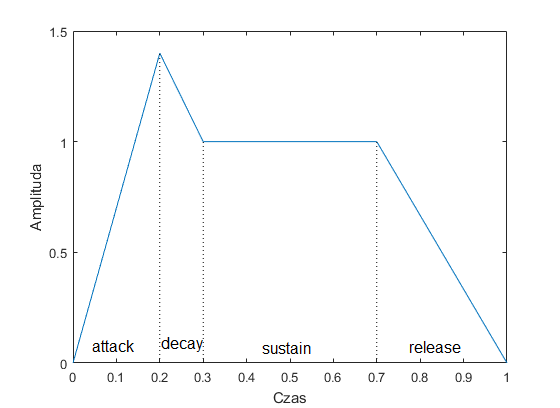
\includegraphics[width=8cm]{./grafiki/real_adsr}
	\captionsetup{justification=centering}
	\caption{Stany ADSR.}
	\label{rys:real_adsr}
\end{figure}
Gdy wciśnięty zostanie klawisz syntezatora, w tablicy stanów ADSR elementowi o indeksie zgodnym z indeksem tablicy freqs[.] (opisaną w \ref{section:real_polifonia}) przypisana zostanie wartość oznaczająca stan "attack". Gdy syntezowany dźwięk jest w tym stanie, wartość obwiedni w tablicy o odpowiednim indeksie jest zwiększana wraz z upływem czasu. Gdy osiągnięta zostanie wartość maksymalna, stan ADSR tego dźwięku zostanie zmieniony na "decay". Wartość obwiedni maleje aż do osiagnięcia ustalonego poziomu dla stanu "sustain". Gdy to nastąpi, stan zostanie zmieniony na "sustain" i będzie on trwał aż do zwolnienia klawisza instrumentu. Zwolnienie klawisza spowoduje przejście do stanu "release" i stopniowe wyzerowanie wartości obwiedni. Po osiągnięciu zera przez wartość obwiedni danego dźwięku, jego stan jest czyszczony, a odpowiedni element tablicy opisanej w \ref{section:real_polifonia} zostaje wyzerowany, co kończy syntezę danego dźwięku.

Użytkownik ma możliwosć ustawiania, za pomocą interfejsu użytkownika, czasu trwania stanów "attack", "decay" i "release" oraz poziomu dla stanu "sustain".

\section{Interfejs użytkownika}
<TODO>